\documentclass[titlepage]{article}
\usepackage[12pt]{extsizes} 
\usepackage[T2A]{fontenc}
\usepackage[utf8]{inputenc}
\usepackage[english,russian]{babel}
%\usepackage{pscyr}
\usepackage{hyperref}
\usepackage{setspace}
\usepackage{amsmath,amssymb,amsfonts,amsthm,secdot}
\usepackage[left=30mm, top=20mm, right=30mm, bottom=20mm, nohead, footskip=15mm]{geometry} 
\usepackage[pdftex]{graphicx}
\usepackage[indentfirst]{titlesec}
\usepackage[usenames]{color}
\usepackage{colortbl}
\usepackage{listings}
\usepackage{secdot}

\def\l{\left}
\def\r{\right}
\def\le{\leqslant}
\def\ge{\geqslant}

\begin{document} 

\newtheorem{theorem}{Теорема}
\newtheorem{lemma}{Лемма}
\newtheorem{definition}{Определение}
\renewcommand{\proofname}{Доказательство}

\begin{center}
\hfill \break
\hfill \break
\hfill \break
\LARGE Приближенное решение дифференциального уравнения \\
\hfill \break
\large Михайлин Д.А. \\
\hfill \break
\today \\

\end{center}

\section{Постановка задачи}
Требуется найти приближенное обобщенное решение задачи
\begin{gather}
	\notag \frac{d}{dx}\l(k(x)\frac{du}{dx}\r) - q(x)u = f(x), 	\ \ x \in [0,10], \ \text{где}
\end{gather}
\begin{gather}
	\notag f(x) = \sin{x} \\
	\notag k(x) = 
		\begin{cases}
			1, x \in [0,3] \cup [7,10] \\
			3, x \in (3,7) 
		\end{cases}
		\\
		\notag q(x) = 
		\begin{cases}
			1, x \in [0,3] \cup [7,10] \\
			3, x \in (3,7)
		\end{cases}
\end{gather}
с краевыми условиями
\begin{gather}
	\notag (k(x)\frac{du}{dx}-0.1u)\Big|_{x = 0} = 0 \\
	\notag u(x)\big|_{x = 10} = 1 
\end{gather}
с точностью $\varepsilon = 10^{-2}$.

Решением данной задачи является такая функция $u$, что функции $u$ и $ku'$ непрерывны на $[0,10]$. Из курса обыкновенных дифференциальных уравнений известно, что при кусочно гладких коэффициентах $k(x), q(x)$ и $f(x)$ данная задача имеет единственное решение. 

\section{Построение разностной схемы для уравнения и краевых условий}
Так как существуют точки разрыва функции $k(x)$ на отрезке $[0 10]$ будем рассматривать интегральное соотношение: 
\begin{gather}
	\notag \int_{x1}^{x2}(q(x)u(x) + f(x))dx = k(x)y'\big|_{x1}^{x2} \\
\end{gather}
Это соотношение должно выполняться для любых $x_1, x_2$ из отрезка $[0, 10]$. Будем искать решение $u(x)$, удовлетворяющее условиям:
\begin{enumerate}
	 \item{ $u(x)$ непрерывна на отрезке $[0, 10]$}
	\item{ $u(x)$ удовлетворяет исходному уравнению всюду, за исключением точек 3 и 7.}
	\item{ Поток $w(x) = k(x)u'(x)$ непрерывен на $[0, 10]$}
\end{enumerate}
Пусть $N \in \mathbb{N}$ -- количество отрезков, на которые разбивается исходный отрезок $[a,b]$. Возьмем шаг $h=\frac{b-a}{N}$, узлы сетки $x_n = a + nh$, $y_n$ -- приближение к значениям $u_n = u(x_n)$. Представим функцию $u(x)$, как $u(x) = u_i + O(h)$, $x - x_i=O(h)$ на отрезке $[x_{i - 1/2},x_{i + 1/2}]$, где $x_{i + 1/2} = x_i + h/2$. Подставим это в выражение выше и проинтегрируем по отрезку $[x_{i - 1/2}, x_{i + 1/2}]$:

\begin{gather}
	\notag \int_{x_{i - 1/2}}^{x_i{i + 1/2}}(q(x)u(x) + f(x))dx = \int_{x_{i - 1/2}}^{x_i{i + 1/2}}(q(x)(u_i + O(h)) + f(x))dx =\\
	\notag \int_{x_{i - 1/2}}^{x_i{i + 1/2}}q(x)u_idx + \int_{x_{i - 1/2}}^{x_i{i + 1/2}}f(x)dx + \int_{x_{i - 1/2}}^{x_i{i + 1/2}}q(x)O(h)dx = h(\tilde{q_i}u_i + \tilde{f_i}) + O(h^2) \\
	\tilde{q_i} = \frac{1}{h}\int_{x_{i - 1/2}}^{x_i{i + 1/2}}q(x)dx \\
	\tilde{f_i} = \frac{1}{h}\int_{x_{i - 1/2}}^{x_i{i + 1/2}}f(x)dx
\end{gather}
Таким образом получаем следующее выражение:
\begin{gather}
	\notag w(x_{i + 1/2}) - w(x_{i - 1/2}) = h(\tilde{q_i}u_i + \tilde{f_i}) + O(h^2)\\
	\notag w(x_{i + 1/2}) - w(x_{i - 1/2})/h  - \tilde{q_i}u_i = \tilde{f_i}  + O(h)
\end{gather}
\begin{gather}
	\notag u'(x) = \frac{w(x)}{k(x)}
\end{gather}
и $w(x) = w(x_{i + 1/2}) + O(h)$ $h = x - x_{i + 1/2}$. Проинтегрируем по отрезку $[x_i,x_{i + 1}]$:
\begin{gather}
	\notag \int_{x_i}^{x_{i + 1}}u'(x)dx = u_{i + 1} - u_i = w(x_{i + 1/2})\int_{x_i}^{x_{i + 1}}\frac{dx}{k(x)} + O(h^2)\\
	\notag \frac{u_{i + 1} - u_{i}}{h} + O(h) = w(x_{i + 1/2})
\end{gather}
где
\begin{gather}
	\notag \tilde{k_{i + 1/2}} = \Big(\frac{1}{h}\int_{x_i}^{x_{i + 1}}\frac{dx}{k(x)}\Big)^{-1}
\end{gather}
Таким образом разностная схема имеет вид:
\begin{gather}
	\notag L_{h}(u)\Big|_{x=x_n} = \frac{\tilde{k_{n + 1/2}}(u_{n + 1} - u_n) - \tilde{k_{n - 1/2}}(u_n - u_{n - 1}}{h^2} - \tilde{q_n}u_n = \tilde{f_n} n = 1, 2...N - 1
\end{gather}
Будем считать, что $N$ нацело делится на $b-a$, тогда коэффициенты $k(x)$ и $q(x)$ постоянны на каждом отрезке $[x_n, x_{n+1}]$. В таком случае, мы можем явно выписать $\tilde{k_{n + 1/2}}, \tilde{q_n} $ и $\tilde f_n$:
\begin{gather}
	\notag \tilde{k}_{n + 1/2} = \Big(\frac{1}{h}\int_{x_i}^{x_{i + 1}}\frac{dx}{k(x)}\Big)^{-1} \\
	\notag \tilde{q}_{n} = \frac{1}{h}\int_{x_i - 1/2}^{x_{i + 1/2}}q(x)dx = \frac{q_{n - 1/2} + q_{n + 1/2}}{2} \\
	\notag \tilde{f}_n = \frac{1}{h}\int_{x_i - 1/2}^{x_{i + 1/2}}f(x)dx= 		\notag \frac{1}{h}(cos(x_{n - 1/2}) - cos(x_{n + 1/2}))
\end{gather}
\section{Порядок аппроксимации}
	Необходимо показать, что:
\begin{gather}
	\notag ||L_h[u]_h - \tilde{f_n}|| = O(h^2)
\end{gather}
Так как можем брать любую норму, возмем следующую:
\begin{gather}
	\notag ||[u]_n|| = h\sum_{n = 0}^{N}|u_n|
\end{gather}
\section{Oценки погрешности аппроксимации граничных условий}
В правой границе аппроксимируем граничное условие следующим образом:
\begin{gather}
	\notag u_0 = 1
\end{gather}
Так как в $x = 10$ краевое условие первого порядка - следовательно аппроксимация точна.\\
Для аппроксимации условия в левом конце воспользуемся формулой Тейлора в точке $x_0$ и подставим в разложение функции u точку $x_1$.
\begin{gather}
	\notag u(x) = u(x_0) + u'(x_0)(x - x_0) + \frac{u''(x_0)}{2}(x - x_0)^2 + O((x -x_0)^3) \\
	\notag u_1 = u_0 - u'(x_0)h + \frac{u''(x_0)}{2}h^2 + O(h^3)\\
	\notag u'(x_0) = \frac{u_0 - u_1}{h} + \frac{u''(x_0)}{2}h + O(h^2)\\
	\notag k_0u'(x_0) - 0.1u_0 = k_0\Big[\frac{u_0 - u_1}{h} + \frac{u''(x_0)}{2}h + O(h^2)\Big] - 0.1u_0 = 0 
\end{gather}
По условию:
\begin{gather}
	\notag u''(x_0) = \frac{q_0u_0 + f_0}{k_0}\\
	\notag k_0\frac{u_0 - u_1}{h} + \frac{q_{0}u_0 + f_0}{2}h - 0.1u_0 = O(h^2)
\end{gather}
Следовательно оценка погрешности имеет второй порядок.
\subsection{Погрешность аппроксимации уравнения}
Рассмотрим сначала такие n, что $x_n$ не попадают в точки разрыва k(x) и q(x). Для таких n на отрезке $[x_{n -1}, x_{n + 1}]$ справедливы следующие равенства:
\begin{gather}
	\notag u_{n + 1} = u_{n} + u'_nh + \frac{u''_n}{2}h^2 + \frac{u'''_n}{6}h^3 + O(h^4)\\
	\notag u_{n - 1} = u_n - u'_nh + \frac{u''_n}{2}h^2 - \frac{u'''_n}{6}h^3 + O(h^4)
\end{gather}
Преобразуем данные разложения следующим образом:
\begin{gather}
	\tilde{k}_{n+1/2} \frac{u_{n + 1} - u_{n}}{h} = \tilde{k}_{n + 1/2}\Big(u'_n + \frac{u''_n}{2}h + \frac{u'''_n}{6}h^2 + O(h^3)\Big) \\
	\tilde{k}_{n - 1/2}\frac{u_n - u_{n - 1}}{h} = \tilde{k}_{n - 1/2}\Big(u'_n - \frac{u''_n}{2}h + \frac{u'''_n}{6}h^2 + O(h^3)\Big)
\end{gather}
Так как k(x) не меняет значения на отрезке $[x_{n - 1}, x_{n + 1}]$ то 
\begin{gather}
	\notag \frac{\tilde{k}_{n + 1/2}(u_{n + 1} - u_n) - \tilde{k}_{n -1/2}(u_n - u_{n - 1})}{h^2} = k_n(u''_n + O(h^2))
\end{gather}
Так как, q(x) не меняет значения на отрезке $[x_{n -1}, x_{n + 1}]$, получим:
\begin{gather}
	\notag L_h(u) - \tilde{f}_n = \frac{\tilde{k}_{n + 1/2}(u_{n + 1} - u_n) - \tilde{k}_{n - 1/2}(u_n - u{n -1})}{h^2} - \tilde{q}_nu_n - \tilde{f}_n = k_nu''_n - q_nu_n - \tilde{f}_n +O(h^2) = \\ f_n - \tilde{f}_n + O(h^2) = O(h^2)
\end{gather}
Покажем, что $ f_n - \tilde{f}_n = O(h^2)$
\begin{gather}
	\notag \tilde{f}_n = \frac{1}{h} \int_{x_{n - 1/2}}^{x_{n + 1/2}}sin(x)dx = \frac{1}{h}(cos(x_{n - 1/2}) - cos(x_{n + 1/2})) \\
	\notag f_n - \tilde{f}_n = sin(x_n) - \frac{1}{h}(cos(x_{n - 1/2}) - cos(x_{n + 1/2})) = \\sin(x_n) - \frac{1}{h}(cos(x_n)cos(\frac{h}{2}) + sin(x_n)sin{\frac{h}{2}} - cos(x_n)cos(\frac{h}{2}) + sin(x_n)sin(\frac{h}{2})) \\
	= sin(x_n) - \frac{2}{h}(sin(x_n)sin(\frac{h}{2})) = \frac{2}{h}sin(x_n)(\frac{h}{2} - sin(\frac{h}{2})) = \frac{2}{h}O(h^3) = O(h^2)
\end{gather}
Рассмотрим теперь такие $n$, что $k(x)$ и $q(x)$ разрывны в точках $x_n$. В $x_n$ функция $u$ имеет непрерывные правые и левые производные, следовательно, можно записать:
\begin{gather*}
	u_{n+1} = u_n + hu_{n,r}' + \frac{h^2}{2}u_{n,r}'' + O(h^3), \\
	u_{n-1} = u_n - hu_{n,l}' + \frac{h^2}{2}u_{n,l}'' + O(h^3), \\
\end{gather*}
где вторые нижние индексы у производных $u$ обозначают правую $(r)$ и левую $(l)$ производные соответственно. Далее:
\begin{gather*}
	\notag \frac{u_{n+1} - u_n}{h} = \l(u_{n,r}' + \frac{h}{2}u_{n,r}'' + O(h^2) \r) \\
	\notag \frac{u_n - u_{n-1}}{h} = \l(u_{n,l}' - \frac{h}{2}u_{n,l}'' + O(h^2) \r)
\end{gather*}
Из условия непрерывности $ku'$ имеем $k_{n+1/2}u_{n,r}' = k_{n-1/2}u_{n,l}'$. Воспользовавшись вышедоказанным равенством $f_n - \tilde f_n = O(h^2)$, получим:
\begin{align*}
	L_{N}(u) - \tilde f_n &= \frac{\tilde{k}_{n + 1/2}(u_{n+1}-u_n) - \tilde{k}_{n - 1/2}(u_n - u_{n-1})}{h^2} - \tilde q_n u_n - \tilde f_n \\ 
	&= \frac{1}{2}(k_{n+1/2}u_{n,r}'' + k_{n-1/2}u_{n,l}'') - \frac{q_{n+1/2}+q_{n-1/2}}{2}u_n - \tilde f_n + O(h) = \\
	&= \frac{1}{2}(k_{n+1/2}u_{n,r}'' - q_{n+1/2}u_n) + \frac{1}{2}(k_{n-1/2}u_{n,l}'' - q_{n-1/2}u_n) - \tilde f_n + O(h) = \\ 
	&= f_n - \tilde f_n + O(h) = O(h)
\end{align*}
Таким образом, в точках разрыва $k(x)$ и $q(x)$ погрешность аппроксимации уравнения составляет $O(h)$. 
Вычислим теперь погрешность аппроксимации в норме $L_1$. В $N-3$ точках погрешность равна $O(h^2)$, а в двух других -- $O(h)$. Тогда погрешность в норме $L_1$ равна:
$$(N-3)hO(h^2) + 2hO(h) = NhO(h^2) + O(h^3) + O(h^2) = O(h^2),$$
то есть разностная схема $(1)$ имеет \textbf{второй порядок аппроксимации.}
\section{Метод прогонки}
\subsection{Описание метода прогонки}
Система уравнений (1), (2), (3) записывается в виде $Ay = b$, где 
\begin{gather}
	\begin{pmatrix}
		-\beta_0 & \gamma_0 & & & & & \\
		\alpha_1 & -\beta_1 & \gamma_1 & & & & \\
		& \alpha_2 & -\beta_2 & \gamma_2 & & & \\
		& & \alpha_3 & -\beta_3 & \ddots & & & \\
		& & & \ddots & \ddots & \gamma_{N-2} & & \\
		& & & & \alpha_{N-1} & \beta_{N-1} & \gamma_{N-1} \\
		& & & & & 0 & 1
	\end{pmatrix}
	, \qquad b = 
	\begin{pmatrix}
		\delta_1 \\ \tilde f_1 \\ \tilde f_2 \\ \vdots \\ \vdots \\ \tilde f_{N-1} \\ 1
	\end{pmatrix}	
\end{gather}
\begin{gather*}
	\beta_0 = \frac{k_0}{h} + \frac{hq_0}{2} - 0.1\\
	\gamma_0 = \frac{k_0}{h} \\
	\delta_1 = \frac{hf_0}{2} \\
	\\
	\alpha_n = \frac{k_{n-1}}{h^2} \\ 
	\beta_n = \frac{k_{n-1} + k_n}{h^2} + \tilde q_n \\
	\gamma_n = \frac{k_n}{h^2}
\end{gather*}
Отметим, что все $\alpha_n, \beta_n, \gamma_n$ $(n = 1,2,\dots,N-1)$ положительны. 

Исключим неизвестные от $y_0$ до $y_{N-1}$. Для этого сначала решим каждое уравнение относительно $y_n$:
\begin{gather}
	\notag y_0 = \frac{\gamma_0}{\beta_0}y_1 - \frac{\delta_1}{\beta_0} \\
		   y_n = C_n y_{n+1} + \varphi_n, \quad n = 0,1,\dots,N-1
\end{gather}
Теперь подставим полученное выражение вместо $y_n$ в следующее уравнение, возникающее вследствие перемножения матрицы $A$ и столбца $\bar y$:
$$(-\beta_{n+1} + \alpha_{n+1}C_n)y_{n+1} + \gamma_{n+1}y_{n+2} = b_{n+1} - \alpha_{n+1}\varphi_n$$
и тем самым получим:
\begin{gather*}
	y_{n+1} = \frac{\gamma_{n+1}}{\beta_{n+1} - \alpha_{n+1}C_n}y_{n+2} + \frac{\alpha_{n+1}\varphi_n - b_{n+1}}{\beta_{n+1} - \alpha_{n+1}C_n} \\
	C_0 = \frac{\gamma_0}{\beta_0}, \quad \varphi_0 = \frac{-\delta_1}{\beta_0} \\
	C_{n+1} = \frac{\gamma_{n+1}}{\beta_{n+1}-\alpha_{n+1}C_n} \\
	\varphi_{n+1} = \frac{\alpha_{n+1}\varphi_n - b_{n+1}}{\beta_{n+1} - \alpha_{n+1}C_n}
\end{gather*}
На последнем шаге получим уравнение:
$$y_{N-1} = C_{N-1}y_N + \varphi_{N-1}$$
Подставим вместо $y_N$ граничное условие:
$$y_{N-1} = C_{N-1}\cdot0 + \varphi_{N-1} = \varphi_{N-1}$$
Остальные $y_n$ находятся в порядке $n = N-2, N-3, \dots, 1, 0$ с использованием (5).

\subsection{Устойчивость метода прогонки}
Докажем устойчивость метода. Под устойчивостью метода будем понимать, что если в процессе вычислений некоторое значение $y_n$ было получено с ошибкой, а дальнейшие вычисления точны, то ошибка в вычисляемых далее $y_n$ не будет увеличиваться.

Как видно из (5), для этого достаточно, чтобы
\begin{gather}
	0 \le C_n \le 1, \quad n = 0,1,\dots,N-1
\end{gather}

\begin{proof}
Докажем формулу (6) по индукции:\\
База индукции: $C_0 = \frac{\gamma_0}{\beta_0}, \ 0 \le C_0 < 1$, так как все $k_0, q_0, h > 0$ \\
Переход индукции. Пусть $0 \le C_n < 1$. Тогда $0 \le C_{n+1} < 1$.
\begin{gather*}
	\gamma_{n+1} + \alpha_{n+1}C_n < \gamma_{n+1} + \alpha_{n+1} < \beta_{n+1} \\
	0 < \gamma_{n+1} < \beta_{n+1} - \alpha_{n+1}C_n \\
	0 < \frac{\gamma_{n+1}}{\beta{n+1} - \alpha_{n+1}C_n} < 1
	0 < C_{n+1} < 1
\end{gather*}
Значит формула (6) доказана и, соответственно, доказана устойчивость метода прогонки.	
\end{proof}

\section{Сходимость}
\begin{theorem}
	Если задача $A_h u_h = F_h$ линейна, то из аппроксимации порядка $k$ и устойчивости метода следует сходимость порядка $k$.
\end{theorem}
\begin{proof}
\hfill \\
Пусть $y$ -- точное решение задачи $A_hy = F_h$, а $u$ -- точное решение приближаемой задачи. \\
Из аппроксимации следует, что $\|A_hu - F_h\| \le C_1h^k$ для некоторого $C_1$, начиная с некоторого $h$. \\
Положим $\tilde F_h = A_h u$. Тогда $\tilde y = [u]_h$ является решением задачи $A_h \tilde y = \tilde F_h$. \\
Из устойчивости метода следует, что:
$$\| y - \tilde y \| \le C_2 \| F_h - \tilde F_h \| = C_2 \| A_h u - F_h \| \le C_1 C_2 h^k$$ 
Таким образом, имеет место сходимость порядка $k$.
\end{proof}

\section{Результаты счёта}
Воспользуемся правилом Рунге. Будем запускать программу для $N = 10,\ 20,\ 40,\dots,10\cdot2^n$, получая численные решения $y^{(10)},\ y^{(20)},\  y^{(40)},\ \dots ,\  y^{(10\cdot2^n)}$, где каждое $y^{(N)} = \{y_i^{(N)}\}_{i=0}^{N}$, пока не найдем такое $N$, что:

\begin{gather*}
	\frac{10}{2N} \l( \sum_{i=1}^{N-1}{\l| y_i^{(N)} - y_{2i}^{(2N)} \r|} + \sum_{i=1}^{N}{ \l| \frac{y_i^{(N)} + y_{i-1}^{(N)}}{2}  - y_{2i-1}^{(2N)} \r|} \r) + \l|y_0^{(N)} - y_{0}^{(2N)}\r| + \l|y_N^{(N)} - y_{2N}^{(2N)}\r| < \varepsilon = 10^{-2}
\end{gather*}

Метод Рунге завершил свою работу при $N = 2048$. График полученного решения представлен ниже на Рис. 1.

\begin{figure}[h]
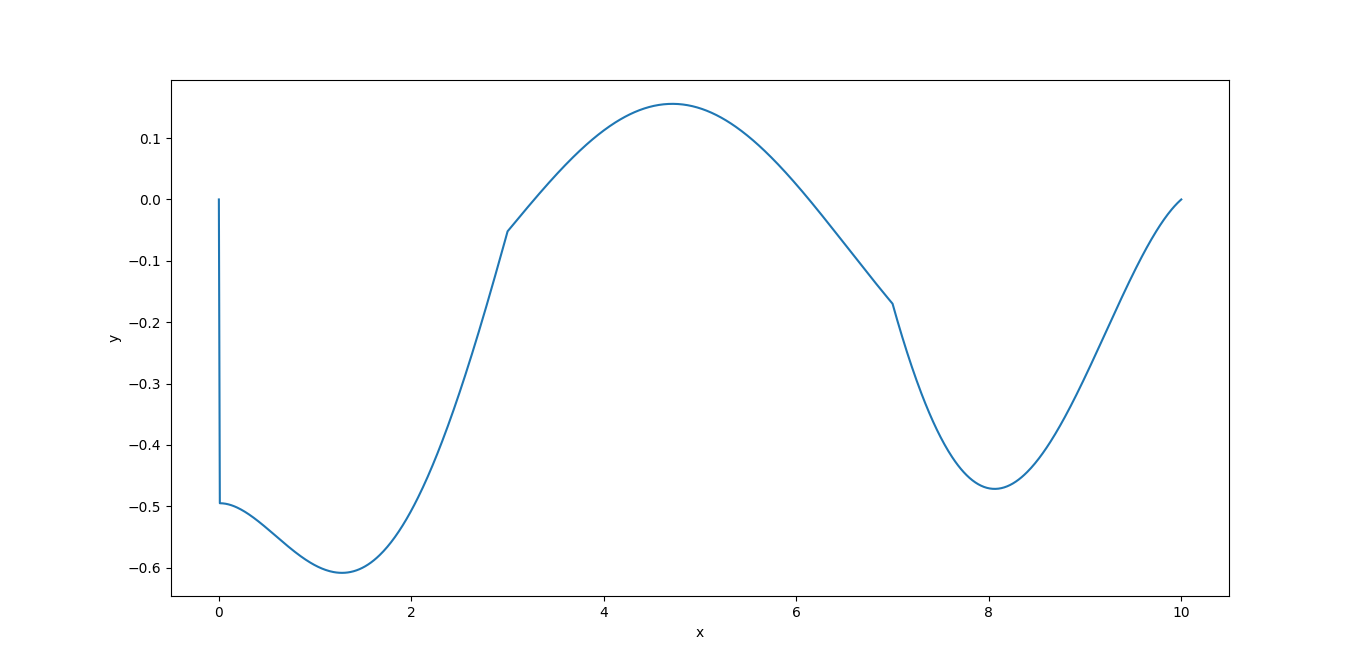
\includegraphics[width=150mm]{Figure_1.png}		
	\caption{График построенного приближенного решения}
\end{figure}
	






\end{document}